%% 
%% Copyright 2019-2020 Elsevier Ltd
%% 
%% This file is part of the 'CAS Bundle'.
%% --------------------------------------
%% 
%% It may be distributed under the conditions of the LaTeX Project Public
%% License, either version 1.2 of this license or (at your option) any
%% later version.  The latest version of this license is in
%%    http://www.latex-project.org/lppl.txt
%% and version 1.2 or later is part of all distributions of LaTeX
%% version 1999/12/01 or later.
%% 
%% The list of all files belonging to the 'CAS Bundle' is
%% given in the file `manifest.txt'.
%% 
%% Template article for cas-dc documentclass for 
%% double column output.

%\documentclass[a4paper,fleqn,longmktitle]{cas-dc}
\documentclass[a4paper,fleqn]{cas-dc}

%\usepackage[authoryear,longnamesfirst]{natbib}
%\usepackage[authoryear]{natbib}
\usepackage[numbers]{natbib}

%%%Author definitions
\def\tsc#1{\csdef{#1}{\textsc{\lowercase{#1}}\xspace}}
\tsc{WGM}
\tsc{QE}
\tsc{EP}
\tsc{PMS}
\tsc{BEC}
\tsc{DE}
%%%
% -------------------------------------------------------------------
% Pacotes para inserção de figuras e subfiguras
\usepackage{subfig,epsfig,tikz,float}		            % Packages de figuras. 
\usepackage{graphicx}
\graphicspath{ {./figs/} }
% -------------------------------------------------------------------
% \usepackage{amssymb}
% -------------------------------------------------------------------
% Pacotes para inserção de tabelas
\usepackage{booktabs,multicol,multirow,tabularx,array}          % Packages para tabela
\usepackage{natbib}
\usepackage{pifont}
\usepackage{xcolor}
% -------------------------------------------------------------------
\PassOptionsToPackage{style=super,nolist}{glossaries}
\PassOptionsToPackage{acronym}{glossaries}
\PassOptionsToPackage{nonumberlist}{glossaries}
\usepackage{glossaries}
\newacronym{ai}{AI}{Artificial Intelligence}
\makeglossaries
% -------------------------------------------------------------------
\usepackage[utf8]{inputenc} % The default since 2018
\DeclareUnicodeCharacter{200B}{{\hskip 0pt}}
% -------------------------------------------------------------------
\begin{document}
\let\WriteBookmarks\relax
\def\floatpagepagefraction{1}
\def\textpagefraction{.001}
\shorttitle{Leveraging social media news}
\shortauthors{CV Radhakrishnan et~al.}


\title [mode = title]{Decentralized File Exchange Hub: A Cloud-Native Approach}                     

\credit{Conceptualization of this study, Methodology, Software}

\author[1]{Rafael Pereira}[type=editor,
                        %auid=000,bioid=1,
                        linkedin='rafaelmendespereira',
                        orcid=0000-0001-8313-7253]
%\cormark[1]
%\fnmark[1]
\ead{rafael.m.pereira@ipleiria.pt}
   
\address[1]{Computer Science and Communications Research Centre, School of Technology and Management, Polytechnic of Leiria, 2411-901 Leiria, Portugal}

\begin{abstract}

The exchange of files has been a fundamental aspect of communication and collaboration throughout the history of computing. From the early days of floppy disks and bulletin board systems to the rise of email attachments and file-sharing platforms, the need to transfer digital files has continued to evolve. In recent years, with the proliferation of cloud-based services and an increasing focus on decentralization, the landscape of file exchange has become more complex and diverse.

In this context, our decentralized file exchange hub aims to revolutionize the way individuals and organizations share and manage files. By leveraging the power of cloud-native technologies and a modular, microservices-based architecture, our system simplifies the file exchange process, providing an intuitive and efficient experience for users. By combining the benefits of a Presentation Provider, an Express File Management Service, an Asynchronous Message Communication Server, and a File Gateway Service, we are able to offer a robust and scalable solution that adapts to the ever-changing demands of the digital world.

With our system in place, users can easily exchange files without worrying about the underlying infrastructure, ensuring that they can focus on their core tasks and projects. As the need for secure, reliable, and efficient file-sharing solutions continues to grow, our decentralized file exchange hub stands as a testament to the potential of modern cloud computing technologies to reshape the landscape of digital collaboration.

\end{abstract}

\begin{keywords}
Decentralized file exchange \sep Microservices architecture \sep Containerization \sep Cloud-native deployment \sep Real-time communication \sep Scalability and resilience
\end{keywords}


\maketitle

\section{Introduction}

The rapid growth of cloud computing and microservices has revolutionized the way applications are developed and deployed. As a result, there is an increasing need for effective strategies to manage the complexity and scalability of these systems. This report explores the design and deployment of a distributed cloud-based application that utilizes containerization and microservices to achieve high availability, performance, and maintainability.

The application is divided into four main modules: Presentation Provider (Nginx), API (Express), Asynchronous Message Communication server, and Database (MongoDB). Each module is designed to serve a specific purpose and can scale independently to adapt to changing loads and requirements. The application also leverages Google Cloud Platform (GCP) services such as Cloud Storage Bucket for storing and managing files.

The report is structured as follows: Section \ref{sec:architecture} presents the architecture of the application, detailing the purpose and design of each module. Section \ref{sec:scenarios} discusses the two scenarios in which our application can be set up and run, namely the local and production scenarios, and outlines their respective architectures and communication patterns. Section \ref{sec:deployment} describes the deployment process, emphasizing the use of GCP's Cloud Build and Cloud Run services to automate and streamline the deployment of the application components. Section \ref{sec:discussion} provides a comprehensive discussion on the different scenarios, difficulties faced during deployments, and offers recommendations for developers working on similar projects. Finally, the report concludes with a summary of the key findings and insights gained from the project.

\section{Architecture}\label{sec:architecture}

This project follows a microservices architecture, which allows for improved scalability, resilience, and maintainability. The system is divided into four main components, each responsible for a specific aspect of the application. Figure \ref{fig:architecture} presents a diagram of the architecture, illustrating the relationship between each component.

\begin{enumerate}
    \item Presentation Provider (Nginx): This component acts as the frontend server, hosting the React web application and serving static files. It is responsible for delivering the user interface to the clients and handling incoming HTTP requests.
    \item API (Express File Management Service): This component is the backend server implemented using Express.js. It manages the file uploading and downloading processes, interacting with the Database and Cloud Storage Bucket to store and retrieve files.
    \item Asynchronous Message Communication Server (Socket.io): This server enables real-time communication between the clients, ensuring that users in the same room receive instant updates when a new file is shared.
    \item Database (MongoDB): The database stores information about the rooms, users, and file metadata, including the bucket URL and timestamp. MongoDB was chosen for its flexibility, scalability, and performance.
    \item Cloud Storage Bucket (Azure Blob Storage): This component stores the uploaded files, providing a reliable and scalable storage solution.
\end{enumerate}

In this architecture, each component communicates with the others through well-defined interfaces, allowing for efficient collaboration and easy maintenance. The use of containerization and cloud-native deployment further enhances the system's scalability and resilience.

\subsection{Presentation Provider: Nginx-based Frontend}

The presentation layer of our file exchange hub is built using a React web application. We utilize Nginx as a reverse proxy and web server to serve the static content generated by the React application. Nginx offers excellent performance, stability, and low resource usage, making it an ideal choice for our frontend. Furthermore, its ability to handle a large number of simultaneous connections ensures a responsive user experience, even during peak loads.

\subsection{API: Express-based File Management Service}

Our file management service is implemented using Node.js with the Express framework, providing a robust and scalable API for managing file metadata and coordinating file transfers. This service is responsible for handling user authentication, managing file metadata, and communicating with the File Gateway service for actual file uploads and downloads. Express is chosen for its ease of use, extensive documentation, and compatibility with Node.js, which allows for efficient development and seamless integration with other components of the File Exchange Hub.

\subsection{Database: MongoDB}

MongoDB, a NoSQL database, is utilized to store information about rooms, files, and users. It's flexible schema and horizontal scalability makes it a fitting choice for our cloud-native application, as it can easily adapt to changing requirements and handle large volumes of data. Additionally, MongoDB provides a rich query language and high-performance indexing capabilities, allowing for efficient data retrieval and manipulation.

\subsection{Asynchronous Message Communication Server: Socket.IO}

To enable real-time communication and notifications within our file exchange hub, we employ Socket.IO, a popular library for real-time web applications. This server facilitates instant messaging between users in the same room, ensuring a seamless and interactive experience for all participants. Socket.IO is selected for its flexibility, reliability, and compatibility with various platforms and transports, making it a powerful solution for real-time communication in our application.

\subsection{File Gateway: Node.js-based File Streaming Service}

The File Gateway service is a Node.js-based application designed to efficiently stream files between clients and the cloud storage service. It acts as an intermediary, managing incoming file requests and delivering the requested files to the clients in real-time. This service ensures optimal performance and reduced latency by employing features such as caching, parallel streaming, and buffering. The File Gateway is built using Node.js for its high-performance capabilities, non-blocking I/O model, and ease of integration with other components, making it an ideal choice for this crucial aspect of the File Exchange Hub.

\subsection{Cloud Storage Bucket: Azure Blob Storage}

To store and manage the actual files exchanged by users, we leverage Azure Blob Storage. This fully managed object storage service offers high availability, durability, and scalability, allowing our file exchange hub to efficiently store, retrieve, and share files. The choice of Azure Blob Storage is driven by its integration with other Azure services, its security features, and its cost-effective pricing model, making it a suitable solution for our application's file storage needs.

\section{Scenarios} \label{sec:scenarios}

In this section, we will discuss the two scenarios in which our application can be set up and run: the local scenario and the production scenario. Each scenario has its own architecture and communication patterns between the different services. Understanding these scenarios helps in setting up, testing, and deploying the application effectively.

\subsection{Local scenario}

In the local scenario, all components are hosted and run locally on the developer's machine. The following diagram (Figure \ref{fig:architectureLocal}) depicts the relationships between the components:

\begin{figure}[h]
\centering
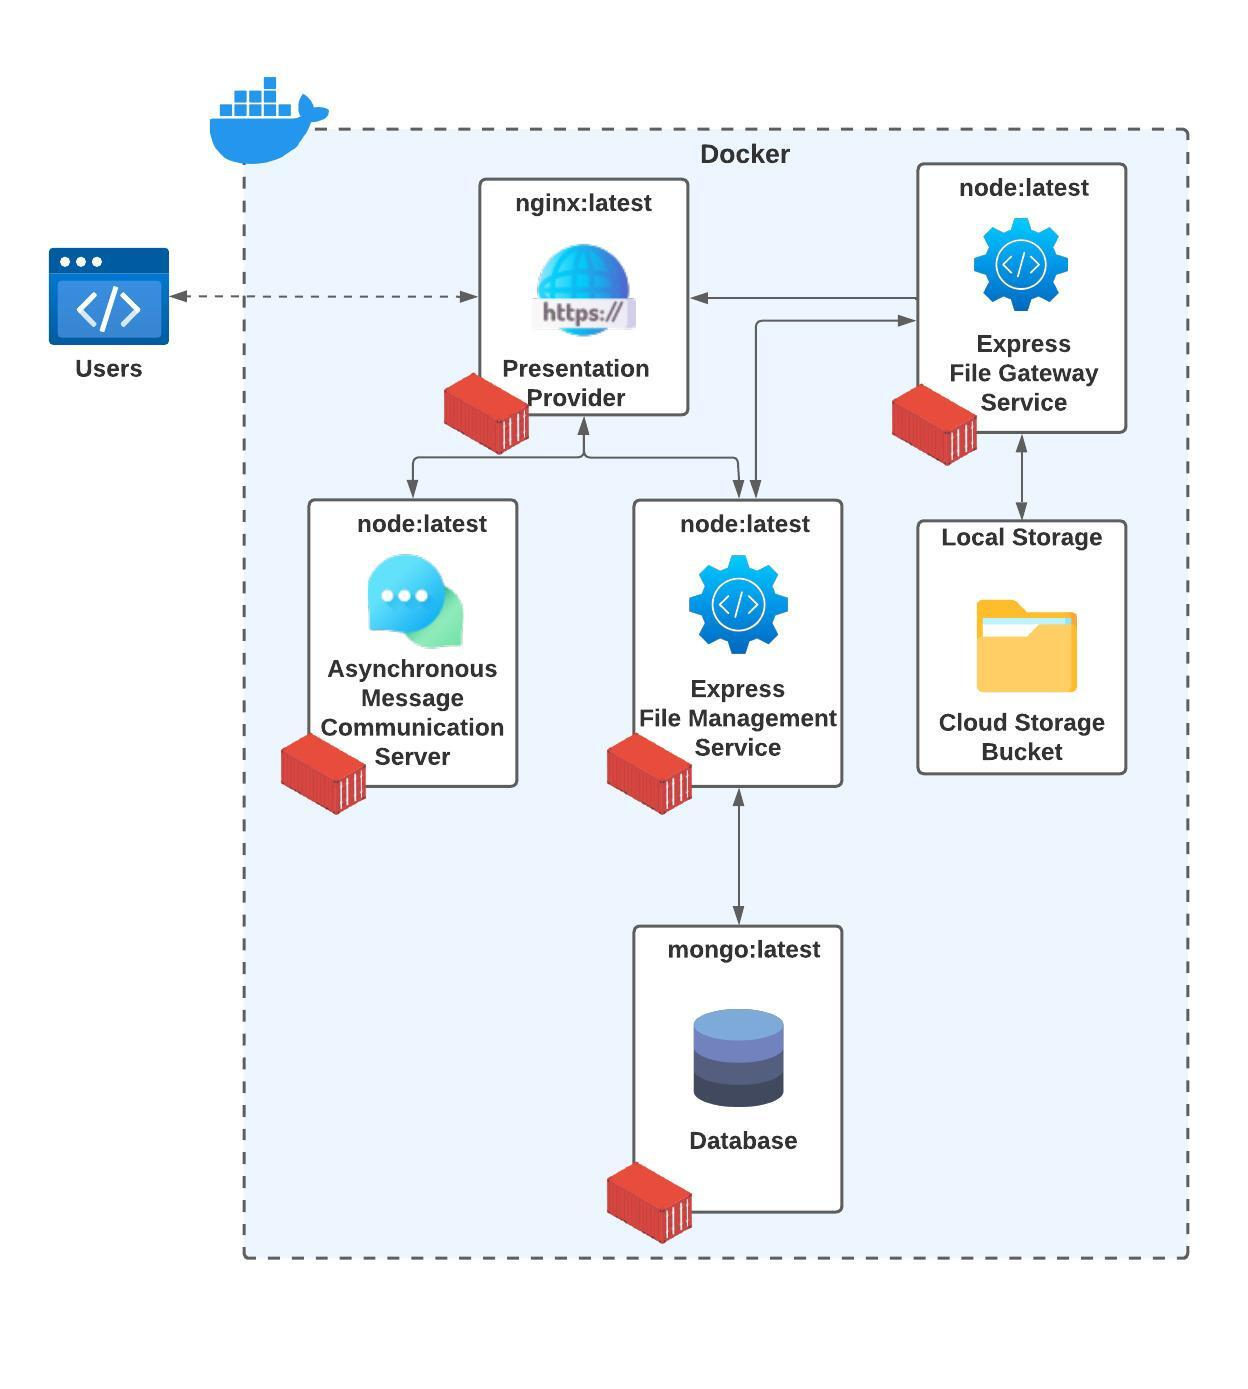
\includegraphics[width=8cm]{architectureLocal.jpeg}
\caption{Local system architecture diagram.}
\label{fig:architectureLocal}
\end{figure}

In this setup, the Presentation Provider communicates directly with the Express File Management Service, Asynchronous Message Communication Server, and File Gateway Service, which are all running on the same local machine. The Express File Management Service is responsible for user authentication and managing file metadata. The Asynchronous Message Communication Server handles real-time communication, and the File Gateway Service manages the actual file uploads and downloads by interacting with the local storage.

\subsection{Production scenario}
In the production scenario, the services are deployed on Google Cloud Run, and the storage is handled by Google Cloud Storage. The following diagram (Figure \ref{fig:architectureProd}) depicts the relationships between the components:

\begin{figure}[h]
\centering
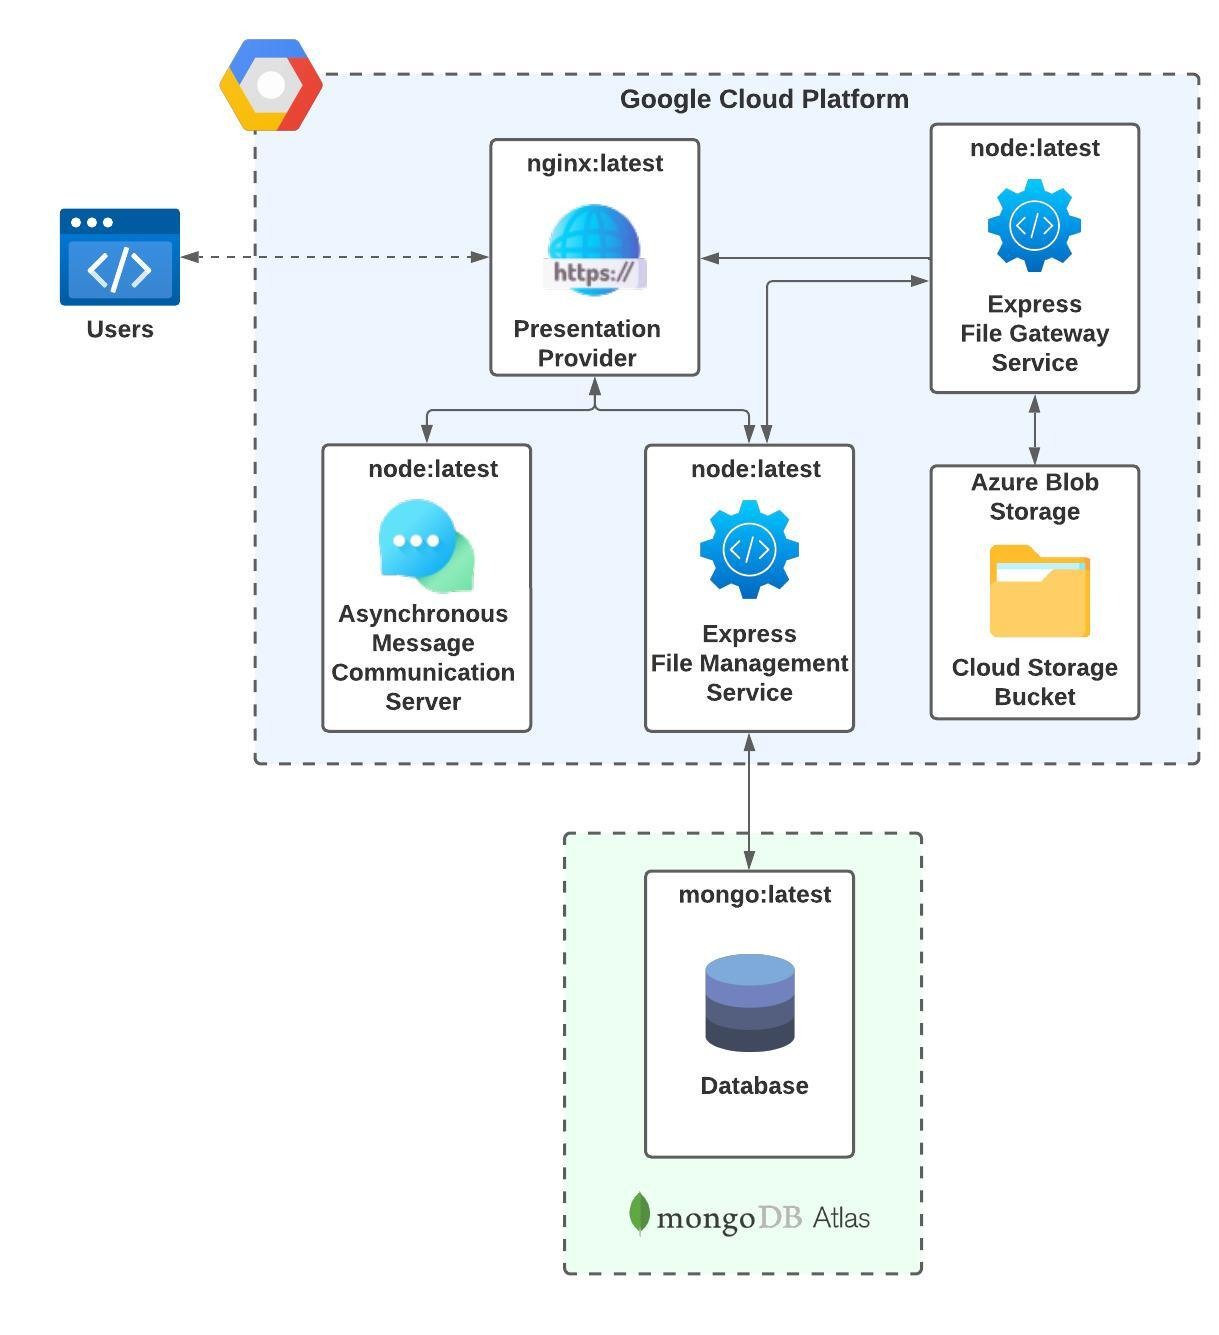
\includegraphics[width=8cm]{architectureProd.jpeg}
\caption{Production system architecture diagram.}
\label{fig:architectureProd}
\end{figure}

In this setup, the Presentation Provider communicates with the Express File Management Service, Asynchronous Message Communication Server, and File Gateway Service through their respective exposed endpoints. The Express File Management Service is responsible for user authentication and managing file metadata. The Asynchronous Message Communication Server handles real-time communication, and the File Gateway Service manages the actual file uploads and downloads by interacting with the Google Cloud Storage. This architecture provides better scalability and reliability, as each service can be independently managed and scaled in response to the system's demands.

\section{Provisioning} \label{sec:deployment}

The deployment process is designed to ensure a smooth transition from development to production, leveraging the power of Google Cloud Platform (GCP) services. The deployment strategy uses GCP's Cloud Run service, along with GitHub Actions, Docker Hub, and Terraform, for automating and streamlining the process. Figure \ref{fig:deployment} presents a diagram of the deployment process, illustrating the steps and relationships between each involved service.

\begin{enumerate}
\item GitHub Actions: This service automates the build and deployment of the application components. It is triggered by a push to the repository, builds the Docker images, and pushes them to Docker Hub.
\item Terraform: Terraform applies the infrastructure changes and triggers Cloud Run to pull Docker images from Docker Hub and deploy the containerized services.
\item Cloud Run: This service deploys the containerized applications on a fully managed platform, providing automatic scaling and load balancing. It ensures that the services are highly available and resilient.
\end{enumerate}

Figure \ref{fig:deployment} depicts the deployment process and the relationships between the components, illustrating the following flow: (1) The developer commits and pushes changes to the repository, (2) which triggers GitHub Actions to (3) build and push Docker images to Docker Hub. (4) Terraform is then initiated, applying infrastructure changes, (5) retrieving and writing the Terraform state to the cloud storage bucket as the remote backend for persistence and collaboration, and (6) subsequently triggering Cloud Run to (7) pull images from Docker Hub and (8) deploy the containerized services.

\begin{figure}[h]
\centering
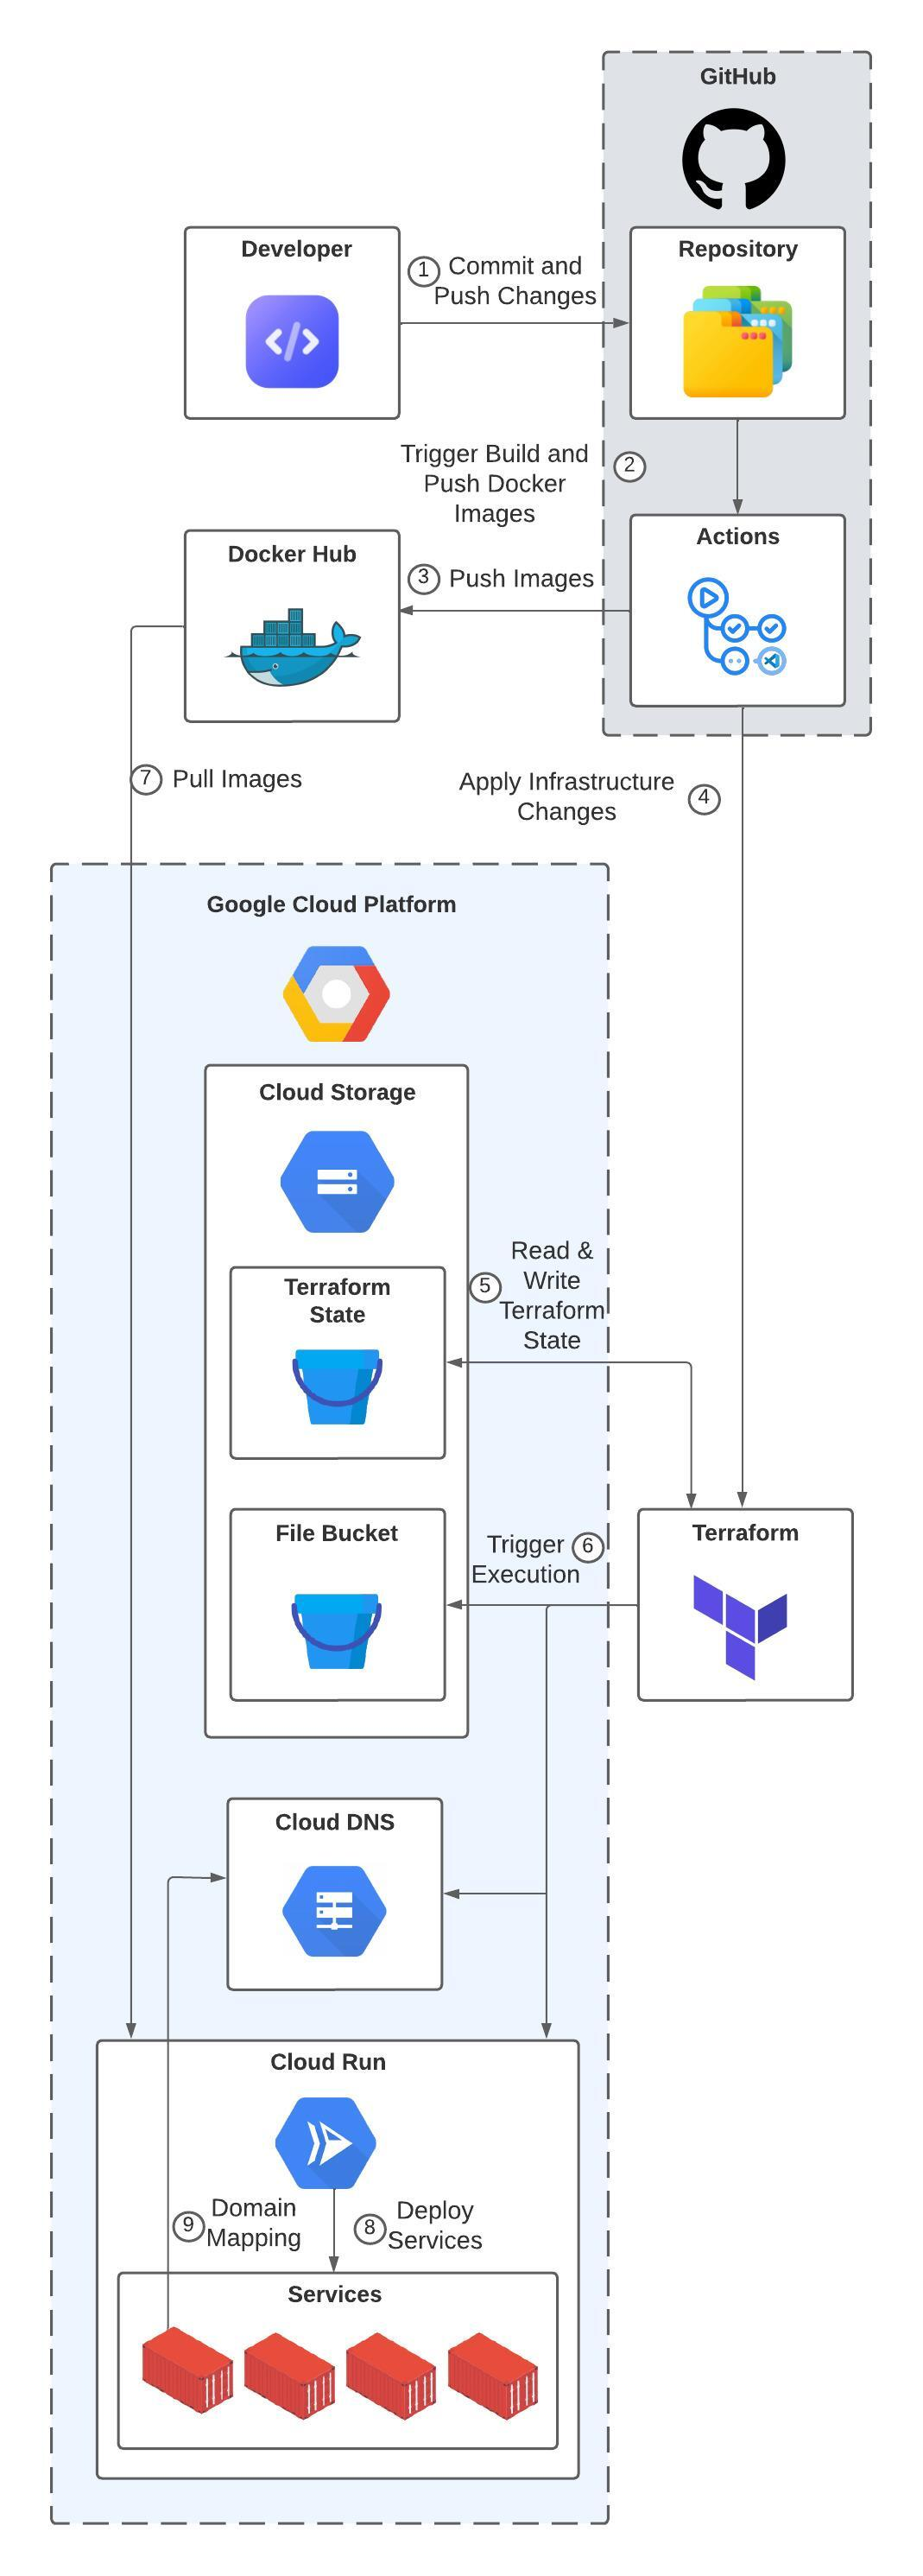
\includegraphics[width=8cm]{provisioning.jpeg}
\caption{Production provisioning process diagram.}
\label{fig:deployment}
\end{figure}


The deployment process ensures that the application components are consistently built and deployed across environments, minimizing human error and facilitating continuous integration and delivery.

\subsection{Automated Continuous Deployment with GitHub Actions and Terraform}

In order to streamline the deployment process and ensure a consistent and efficient release cycle, we implemented Continuous Deployment using GitHub Actions and Terraform. GitHub Actions automates the process of building and pushing Docker images to Docker Hub, while Terraform manages the infrastructure required to deploy and update the services on Google Cloud Run.

When changes are pushed to the repository, GitHub Actions triggers an automated workflow that builds and pushes the updated Docker images for each microservice to Docker Hub. Following the successful completion of this step, the workflow then initiates the Terraform CLI to manage the deployment of the microservices to Google Cloud Run.

Using Terraform, we define the infrastructure for each microservice as code, including Google Cloud Run services and IAM policies. This approach enables us to maintain a version-controlled and easily auditable infrastructure while also allowing for seamless updates and configuration changes. By integrating with GitHub Actions, we ensure that every push to the repository automatically triggers a new deployment, resulting in a streamlined and consistent release process.

\subsection{Cloud Run: Scalable Containerized Services}

Google Cloud Run is a serverless platform that enables the deployment and management of containerized applications. By leveraging the power of containers, Cloud Run allows developers to focus on writing code without worrying about the underlying infrastructure. The platform automatically scales applications based on demand, ensuring optimal resource usage and minimizing costs.

\section{Discussion} \label{sec:discussion}

Throughout the development of our decentralized file exchange hub, we encountered various challenges and learned valuable lessons about deploying applications both locally and in the cloud. In this section, we will discuss the different scenarios, difficulties faced during deployments, and offer recommendations for other developers embarking on similar projects.

Comparing the local and production scenarios, we noticed that while local deployment is easier to set up and manage, it lacks the scalability and reliability offered by cloud deployment. In the local scenario, all components run on the developer's machine, which simplifies communication between services but limits the system's ability to handle high loads and provide high availability. On the other hand, deploying our application to the cloud using Google Cloud Run and Google Cloud Storage enables us to achieve better scalability and reliability while maintaining a modular architecture. This approach allows each service to be independently managed, scaled, and updated, thus improving the system's overall resilience and flexibility.

During the deployment process, we faced several challenges, including configuring the services to communicate effectively with each other, optimizing the containerization process, and ensuring security across all components. To overcome these challenges, we relied heavily on documentation, best practices, and online resources, which proved invaluable in guiding our development efforts. Additionally, we learned the importance of thoroughly testing each service independently and as a part of the larger system to ensure seamless integration and functionality.

\section{Conclusion}

This report has presented a decentralized file exchange hub designed with a cloud-native approach. By leveraging containers, microservices, and cloud services, we have created a scalable, resilient, and efficient system for exchanging files. Our use of modern technologies such as Nginx, Express, Socket.IO, MongoDB, and Google Cloud Platform services demonstrates the power and flexibility of cloud computing for modern software applications. Additionally, the integration of GitHub Actions, Google Cloud Build, Terraform, and Google Cloud Run has streamlined the deployment process, providing a robust Continuous Integration and Continuous Deployment (CI/CD) pipeline for ensuring consistent and reliable application delivery. The decentralized file exchange hub showcases the potential for creating high-performance, scalable, and flexible systems using cutting-edge cloud technologies and best practices.

%% Loading bibliography style file
%\bibliographystyle{model1-num-names}
%\bibliographystyle{cas-model2-names}
%\bibliographystyle{unsrt} % Estilo de Bibliografia
% Loading bibliography database
%\bibliography{cas-refs}


%\vskip3pt

\end{document}
